%!TEX TS-program = pdflatex
%!TEX encoding = utf8
\documentclass[12pt, oneside]{book}
\usepackage[T1]{fontenc}
\usepackage[utf8]{inputenc}
\usepackage[english]{babel}
%% FONTS: libertine+biolinum+stix
\usepackage[mono=false]{libertine}
\usepackage[
backend=bibtex,
style=phys,
citestyle=numeric,
sorting=none
]{biblatex}

\addbibresource{references.bib}

% =====================
% = Datos importantes =
% =====================
% hay que rellenar estos datos y luego
% ir a \begin{document}

\title{Simulation and implementation of a Conformal Finite Difference Time Domain method}
\author{Carlos Julio Ramos Salas}
\date{30 Junio 2024}
\newcommand{\tutores}[1]{\newcommand{\guardatutores}{#1}}
\tutores{Dr. Luis Manuel Díaz Angulo}

% ======================
% = Páginas de títulos =
% ======================
\makeatletter
\edef\maintitle{\@title}
\renewcommand\maketitle{%
  \begin{titlepage}
      \vspace*{1.5cm}
      \parskip=0pt
      \Huge\bfseries
      \begin{center}
          \leavevmode
\includegraphics[totalheight=6cm]{Imagenes/sello.jpg}\\[2cm]
          \@title
      \end{center}
      \vspace{1cm}
      \begin{center}
          \@author
      \end{center}
  \end{titlepage}
  
  \begin{titlepage}
  \parindent=0pt
  \begin{flushleft}
  \vspace*{1.5mm}
  \setlength\baselineskip{0pt}
  \setlength\parskip{0mm}
  \begin{center}
      \leavevmode
\includegraphics[totalheight=4.5cm]{Imagenes/sello.jpg}
  \end{center}
  \end{flushleft}
  \vspace{1cm}
  \bgroup
  \Large \bfseries
  \begin{center}
  \@title
  \end{center}
  \egroup
  \vspace*{.5cm}
  \begin{center}
  \@author
  \end{center}
  \vspace*{1.8cm}
  \begin{flushright}
  \begin{minipage}{8.45cm}
      Memoria del {\bf Trabajo Fin de Máster}.\\ 
      Máster en Física y Matemáticas (FisyMat) \\ 
      University of Granada (UGR).

      \vspace*{7.5mm}

      Tutored by:
      % \vspace*{5mm}
  \end{minipage}\par
  \begin{tabularx}{8.45cm}[b]{@{}l}
      \guardatutores
  \end{tabularx}
   \end{flushright}
      \vspace*{\fill}
   \end{titlepage}
   %%% Esto es necesario...
   \pagestyle{tfg}
   \renewcommand{\chaptermark}[1]{\markright{\thechapter.\space ##1}}
   \renewcommand{\sectionmark}[1]{}
   \renewcommand{\subsectionmark}[1]{}
  }
\makeatother

% ======================================
% = Color de la Universidad de Sevilla =
% ======================================
\usepackage{tikz}
\definecolor{USred}{cmyk}{0,1.00,0.65,0.34}

% =========
% = Otros =
% =========
\usepackage[]{tabularx}
\usepackage[]{enumitem}
\setlist{noitemsep}

% ==========================
% = Matemáticas y teoremas =
% ==========================
\usepackage[]{amsmath}
\usepackage[]{amsthm}
\usepackage[]{mathtools}
\usepackage[]{bm}
\usepackage[]{thmtools}
\newcommand{\marcador}{\vrule height 10pt depth 2pt width 2pt \hskip .5em\relax}
\newcommand{\cabeceraespecial}{%
    \color{USred}%
    \normalfont\bfseries}
\declaretheoremstyle[
    spaceabove=\medskipamount,
    spacebelow=\medskipamount,
    headfont=\cabeceraespecial\marcador,
    notefont=\cabeceraespecial,
    notebraces={(}{)},
    bodyfont=\normalfont\itshape,
    postheadspace=1em,
    numberwithin=chapter,
    headindent=0pt,
    headpunct={.}
    ]{importante}
\declaretheoremstyle[
    spaceabove=\medskipamount,
    spacebelow=\medskipamount,
    headfont=\normalfont\itshape\color{USred},
    notefont=\normalfont,
    notebraces={(}{)},
    bodyfont=\normalfont,
    postheadspace=1em,
    numberwithin=chapter,
    headindent=0pt,
    headpunct={.}
    ]{normal}
\declaretheoremstyle[
    spaceabove=\medskipamount,
    spacebelow=\medskipamount,
    headfont=\normalfont\itshape\color{USred},
    notefont=\normalfont,
    notebraces={(}{)},
    bodyfont=\normalfont,
    postheadspace=1em,
    headindent=0pt,
    headpunct={.},
    numbered=no,
    qed=\color{USred}\marcador
    ]{demostracion}

% Los nombres de los enunciados. Añade los que necesites.
\declaretheorem[name=Observaci\'on, style=normal]{remark}
\declaretheorem[name=Corolario, style=normal]{corollary}
\declaretheorem[name=Proposici\'on, style=normal]{proposition}
\declaretheorem[name=Lema, style=normal]{lemma}

\declaretheorem[name=Teorema, style=importante]{theorem}
\declaretheorem[name=Definici\'on, style=importante]{definition}

\let\proof=\undefined
\declaretheorem[name=Demostraci\'on, style=demostracion]{proof}


% ============================
% = Composición de la página =
% ============================
\usepackage[
    a4paper,
    textwidth=80ex,
]{geometry}

\linespread{1.069}
\parskip=10pt plus 1pt minus .5pt
\frenchspacing
% \raggedright


% ==============================
% = Composición de los títulos =
% ==============================

\usepackage[explicit]{titlesec}

\newcommand{\hsp}{\hspace{20pt}}
\titleformat{\chapter}[hang]
    {\Huge\sffamily\bfseries}
    {\thechapter\hsp\textcolor{USred}{\vrule width 2pt}\hsp}{0pt}
    {#1}
\titleformat{\section}
  {\normalfont\Large\sffamily\bfseries}{\thesection\space\space}
  {1ex}
  {#1}
\titleformat{\subsection}
  {\normalfont\large\sffamily}{\thesubsection\space\space}
  {1ex}
  {#1}

% =======================
% = Cabeceras de página =
% =======================
\usepackage[]{fancyhdr}
\usepackage[]{emptypage}
\fancypagestyle{plain}{%
    \fancyhf{}%
    \renewcommand{\headrulewidth}{0pt}
    \renewcommand{\footrulewidth}{0pt}
}
\fancypagestyle{tfg}{%
    \fancyhf{}%
    \renewcommand{\headrulewidth}{0pt}
    \renewcommand{\footrulewidth}{0pt}
    \fancyhead[LE]{{\normalsize\color{USred}\bfseries\thepage}\quad
                    \small\textsc{\MakeLowercase{\maintitle}}}
    \fancyhead[RO]{\small\textsc{\MakeLowercase{\rightmark}}%
                    \quad{\normalsize\bfseries\color{USred}\thepage}}%
                    }

% =============================
% = El documento empieza aquí =
% =============================
\begin{document}


\maketitle

\frontmatter
\tableofcontents

\mainmatter


\chapter*{Acknowledgments}
\addcontentsline{toc}{chapter}{Acknowledgments}
\markright{Acknowledgments}

I would like to thank the "Fundación Carolina", this would be impossible without the opportunity they gave to me. Thanks to my best friends Mario Sánchez and Ana Mejía for their unconditional company. I would also like to thank my tutor Luis Díaz for guiding me in this area of research and welcoming me to this country. 

\indent Finally and most importantly, I would like to thank my parents Margot Salas and Julio Ramos, I am the person I am today thanks them.

\chapter*{English Abstract}
\addcontentsline{toc}{chapter}{English Abstract}
\markright{English Abstract}

Some differential equations in the literature present arduous work to find the associated solution, even in some cases, the solution to said systems turn out to be impossible to find through analytical methods. In this situation, numerical methods plays an important role since the allow us to solve the system of interest through discrete operations with a low numerical error involved.

\indent Among the numerous existing techniques to solve electromagnetism problems, the Finite Difference in Time Domain method (FDTD) stands out, however, when we consider complicated geometries, it is necessary to refine the method in search of better efficiency, that is where we can introduce the Conformal Finite Difference in Time Domain method (CFDTD), which can be studied as the modification of the FDTD by introducing a Perfect Electric Conductor (PEC) volume into the geometry to consider.

\indent In this work, a simulation and implementation of the CFDTD method is made in both one and two dimensions, in the last one, considering a line or an area of PEC that interrupts the spatial mesh worked. The codes worked out were prepared with test-oriented development in the python language, these can be found in the associated GitHub repository presented in annexes.  

\chapter*{Resúmen en Español}
\addcontentsline{toc}{chapter}{Resumen en Español}
\markright{Resúmen en Español}

\begin{otherlanguage*}{spanish}
    \indent Algunas ecuaciones diferenciales en la literatura presentan un trabajo arduoso para encontrar la solución asociada, incluso en algunos casos, la solución a dicho sistema resulta ser imposible de encontrar a través de métodos analíticos. Ante esta situación los métodos numéricos juegan un papel importante ya que nos permiten resolver el sistema de interés a través de operaciones discretas con un bajo error numérico de por medio. 

    \indent Entre las diversas técnicas existentes para poder resolver problemas de electromagnetismo destaca el método de diferencias finitas en el dominio del tiempo (FDTD por sus siglas en inglés), sin embargo, al momento de considerar geometrías complicadas, es necesario refinar el método en búsqueda de una mayor eficiencia, allí es donde se puede introducir la técnica conforme de diferencias finitas (CFDTD), la cual puede ser estudiada como la modificación de FDTD al introducir un volumen de conductor eléctrico perfecto (PEC) en la geometría a considerar.

    \indent En el presente trabajo se realiza una simulación e implementación del método CFDTD tanto en una como en dos dimensiones, en este último caso, considerando una línea o un área de PEC que interrumpen en el mallado. Los códigos trabajados fueron realizados con desarrollo orientado por tests en el lenguaje python, estos pueden encontrar en el repositorio de GitHub asociado presentado en anexos.
\end{otherlanguage*}

\chapter{Introduction}

IDK what to write down here

\chapter{Maxwell's equations and the FDTD method}

Let's first start by introducing the Maxwell's equation of electromagnetism and the basic notions of the FDTD algorithm in one and two dimensions in the free space case.

\section{Introduction to the finite differences}

We want to find a function that is the solution to a specific differential equation, however, this is a hard problem in general and only rarely can an analytic formula be found for the solution. A finite difference method proceeds by replacing the aderivatives in the differential equation with finite differences aproximations \cite{LeVeque,Burden-2016}. For example, let's consider the Taylor approximation for $f(x+h)$ and $f(x-h)$
\begin{align}
    f(x+h) &= f(x) + h  f'(x) + \dfrac{h^2}{2}f''(x) + \mathcal{O}(h^3) = f(x) + h  f'(x) + \mathcal{O}(h^2), \label{eq:taylorFD1}\\
    f(x-h) &= f(x) - h  f'(x) + \dfrac{h^2}{2}f''(x) + \mathcal{O}(h^3) = f(x) - h  f'(x) + \mathcal{O}(h^2),
    \label{eq:taylorFD2}
\end{align}
in both equations it is possible to isolate the derivative, then we obtain:
\begin{align}
    f'(x) &= \dfrac{f(x+h)+f(x)}{h} + \mathcal{O}(h), \\
    f'(x) &= \dfrac{f(x)-f(x-h)}{h} + \mathcal{O}(h).
\end{align}
If we ignore the order $h$ terms, we obtain the first order approximation for the derivative of the function with an error proportional to $h$. However, if we want to improve and reduce the error to order $h^2$, it's necessary to introduce the central finite difference approximation. If we consider $h=\Delta x/2$ and substract the equations \ref{eq:taylorFD1} and \ref{eq:taylorFD2} we can obtain the central finite difference as it follows
\begin{equation}
    f'(x) = \dfrac{f\left( x+ \dfrac{\Delta x}{2} \right) - f\left( x - \dfrac{\Delta x}{2} \right)}{\Delta x} + \mathcal{O}(\Delta x^2),
\end{equation}
we obtain then the approximation searched by ignoring the cuadratic order tearms. Since the error decreases faster in this case for smaller $\Delta x$, the equation will be more efficient to work with, for this reason, this approximation will be used for the discretization of the Maxwell's equations.

\section{One dimensional discrete Maxwell equations}

First let's remember the time-dependent Maxwell's curl equations for free space \cite{jackson, griffiths}
\begin{align}
    &\frac{\partial \boldsymbol{E}}{\partial t}=\frac{1}{\varepsilon_{0}} \nabla \times \boldsymbol{H}, \\
    &\frac{\partial \boldsymbol{H}}{\partial t}=-\frac{1}{\mu_{0}} \nabla \times \boldsymbol{E},
\end{align}
here $\boldsymbol{E}$ and $\boldsymbol{H}$ are vectors in three dimensions, with all the components being functions that depend of the spatial coordinates. For the one-dimensional case we can assume that the only non zero components of $\boldsymbol{E}$ and $\boldsymbol{H}$ are $E_x$ and $H_y$ respectively, then, the previous equations become
\begin{align}
    & \frac{\partial E_x}{\partial t}=-\frac{1}{\epsilon_0}  \frac{\partial H_y}{\partial z}, \\
    & \frac{\partial H_y}{\partial t}=-\frac{1}{\mu_0} \frac{\partial E_x}{\partial z}.
\end{align}
These equations represents a plane wave traveling through the $z$ direction. Taking the central difference approimation discused above for both the temporal and spatial derivatives we obtain \cite{Sullivan2020}
\begin{align}
    \frac{E_x^{n+\frac{1}{2}}(k)-E_x^{n-\frac{1}{2}}(k)}{\Delta t} &=-\frac{1}{\epsilon_0}\frac{H_y^n \left(k+\frac{1}{2}\right) - H_y^n\left(k-\frac{1}{2}\right)}{\Delta x}, \\
    \frac{H_y^{n+1} \left(k+\frac{1}{2}\right) -H_y^{n}\left( k +\frac{1}{2}\right)}{\Delta t} &=-\frac{1}{\mu_0}\frac{E_x^{n+\frac{1}{2}} \left(k+1\right) - E_x^{n+\frac{1}{2}}\left(k\right)}{\Delta x}.
\end{align}
In these two equations, the time step is represented by the superscripts ($n$) while the argument inside functions represent the spatial step ($k$), so the current time and distance are given by $t = \Delta t \cdot n$ and $z = \Delta x \cdot k$. Finally, we can rearrenge the last equations to obtain the next iterative equations
\begin{align}
    E_{x}^{n+1 / 2}(k) &=E_{x}^{n-1 / 2}(k)-\frac{\Delta t}{\varepsilon_{0} \cdot \Delta x}\left[H_{y}^{n}\left(k+\frac{1}{2}\right)-H_{y}^{n}\left(k-\frac{1}{2}\right)\right], \\
    H_{y}^{n+1}\left(k+\frac{1}{2}\right) &=H_{y}^{n}\left(k+\frac{1}{2}\right)-\frac{\Delta t}{\mu_{0} \cdot \Delta x}\left[E_{x}^{n+1 / 2}(k+1)-E_{x}^{n+1 / 2}(k)\right].
\end{align}
It's important to notice that this formulation assume that the electric and magnetic fields are interleaved in both space and time, this is illustrated in the Figure \ref{fig:sullivaninterleaved}.
\begin{figure}[h]
    \centering
    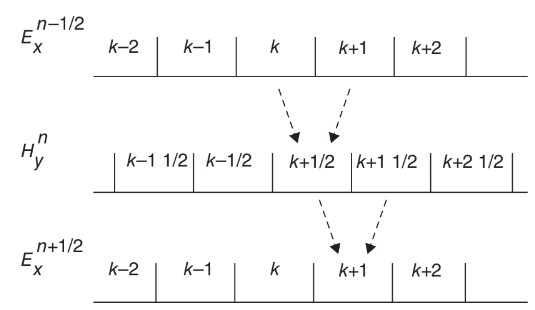
\includegraphics[scale=0.8]{Imagenes/Sullivan_interleaved.jpg}
    \caption{Interleaving of the electric and magnetic fields in the FDTD formulation. Image taken from \cite{Sullivan2020}.}
    \label{fig:sullivaninterleaved}
\end{figure}

% \chapter{Los enunciados}

% \section{Teoremas y demostraciones}


% \begin{theorem}[Euclides]\label{thm:th1}
%     Esto es un Teorema. Se numeran a partir del 1 en cada capítulo. Como son importantes, tienen un cuadrado rojo al principio. Llevan letra cursiva.
% \end{theorem}

% \begin{proof}
%     Esto es la demostración. Al final de la demostración se puede ver un cuadrado rojo similar al de los teoremas. Las demostraciones no llevan letra cursiva.
% \end{proof}


% \begin{definition}\label{def:1}
%     Esto es una definición. Las definiciones son importantes; también llevan un cuadradito rojo.
% \end{definition}


% \subsection{Otros enunciados}


% \begin{remark}
%     Esto es una observación, que dice que $e=mc^{2}$. Como las observaciones no son importantes, no llevan cuadrado rojo, y el tipo de letra no es cursiva.
% \end{remark}


% \begin{proof}
%     Si la demostración acaba en una fórmula, para poner el cuadrado rojo a la altura de la última formula, hay que usar la orden \verb|\qedhere|, como en este caso:
%     \[
%         e=mc^{2}.\qedhere
%     \]

% \end{proof}


% \begin{corollary}\label{cor:1}
%     Esto es un corolario.
% \end{corollary}

% \begin{proposition}\label{pro:1}
%     Esto es una proposición.
% \end{proposition}

% \begin{lemma}[Gauss]\label{lem:1}
%     Esto es un lema.
% \end{lemma}



% \bibliographystyle{plain}
% \biliography{references} 

\chapter{References}
\nocite{*}
%------------------------------------------------------------
\printbibliography[heading=none]

\end{document}